\documentclass{beamer}

\usepackage[english]{babel}

% Font imports and settings
\usepackage{fontspec}
\usepackage{xunicode}
\usepackage{xltxtra}
\defaultfontfeatures{Mapping=tex-text,Scale=MatchLowercase}
\setmainfont[Scale=.95]{HelveticaNeue}
\setsansfont[Scale=.95]{HelveticaNeue}
\setmonofont[Scale=0.65]{Envy Code R}

% Needed packages
\usepackage{hyperref}
\usepackage{verbatim}
\usepackage{listings}
\usepackage{color}
\usepackage{textcomp}
\usepackage{caption}

% Code listing settings
\definecolor{listinggray}{gray}{0.9}
\definecolor{lbcolor}{rgb}{0.95,0.95,0.95}
\definecolor{lightgray}{rgb}{.9,.9,.9}
\definecolor{darkgray}{rgb}{.4,.4,.4}
\definecolor{purple}{rgb}{0.65, 0.12, 0.82}

\captionsetup{labelformat=empty,labelsep=none,font=it}

\lstdefinelanguage{JavaScript}{
  keywords={typeof, new, true, false, catch, function, return, null, catch, switch, var, if, in, while, do, else, case, break},
  keywordstyle=\color{blue}\bfseries,
  ndkeywords={class, export, boolean, throw, implements, import, this},
  ndkeywordstyle=\color{darkgray}\bfseries,
  identifierstyle=\color{black},
  sensitive=false,
  comment=[l]{//},
  morecomment=[s]{/*}{*/},
  commentstyle=\color{purple}\ttfamily,
  stringstyle=\color{red}\ttfamily,
  morestring=[b]',
  morestring=[b]"
}

\lstset{
   language=JavaScript,
   backgroundcolor=\color{lightgray},
   extendedchars=true,
   basicstyle=\ttfamily,
   showstringspaces=false,
   showspaces=false,
   numbers=none,
   tabsize=2,
   breaklines=true,
   showtabs=false,
   captionpos=b
}

\mode<presentation>

\usetheme{default}
\setbeamercovered{dynamic}

% Color settings
\definecolor{iterateblue}{rgb}{0,0.43,0.67} % Definition of yellow color
\setbeamercolor{titlelike}{fg=iterateblue}
\setbeamercolor{structure}{fg=iterateblue}
\setbeamercolor{inverted}{bg=iterateblue,fg=white}

\setbeamertemplate{sidebar right} {}
\setbeamertemplate{navigation symbols}{}
\setbeamertemplate{headline}{
    \begin{beamercolorbox}{inverted}
        \vskip0.1cm
        \hfill
        \llap{\insertlogo\hskip0.1cm}
        \vskip0.1cm
    \end{beamercolorbox}
}

\pgfdeclareimage[interpolate=true,height=0.7cm]{logo}{iterate-logo-white}
\logo{\pgfuseimage{logo}}

\AtBeginSubsection[]
{
  \begin{frame}<beamer>{Agenda}
    \tableofcontents[currentsection,currentsubsection]
  \end{frame}
}

% If you wish to uncover everything in a step-wise fashion
%\beamerdefaultoverlayspecification{<+->}

\begin{document}

\setbeamercolor{background canvas}{bg=iterateblue}
\begin{frame}
    \begin{beamercolorbox}[ignorebg]{inverted}
    \begin{center}
        \Huge{git rebase}\\
        \vspace{0.5cm}
        \large{\emph{ta kontrollen over historien}}\\
        \vspace{1cm}
        \small{Pål Ruud - JavaZone 13. sep 2012}
    \end{center}
    \end{beamercolorbox}%
\end{frame}
\setbeamercolor{background canvas}{bg=white}

\begin{frame}{Innhold}
    \begin{itemize}
        \item Hva er problemet?
        \item Hva er galt med \lstinline$merge$?
        \item Avmystifisering av \lstinline$rebase$.
        \item En enkel arbeidsflyt.
        \item Lek med \lstinline$--interactive$.
    \end{itemize}
\end{frame}

\begin{frame}{Motivasjon}
    \setbeamercovered{invisible}
    \begin{center}
        \texttt{Merge made by the 'recursive' strategy.}\\
        \pause
        ..ti ganger etterhverandre.
        \medskip
        \pause
        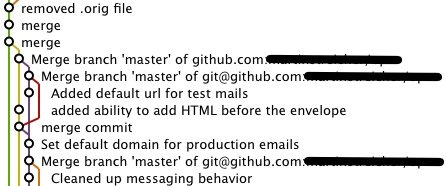
\includegraphics[scale=0.7]{merge_commits.jpg}
    \end{center}
\end{frame}

\begin{frame}{Et vanlig utgangspunkt}
    \begin{center}
        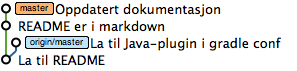
\includegraphics[scale=0.7]{1.png}
    \end{center}
\end{frame}

\begin{frame}[fragile]{}
    \setbeamercovered{invisible}
    \begin{lstlisting}[language=bash]
      $ git pull origin master
    \end{lstlisting}
    \medskip
    \pause
    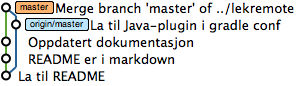
\includegraphics[scale=0.7]{2.png}
\end{frame}

\begin{frame}[fragile]{Hva gjør egentlig \texttt{pull}?}
    \begin{lstlisting}[language=bash]
      $ git pull origin master
    \end{lstlisting}
    \medskip
    ...er det samme som ...
    \medskip
    \begin{lstlisting}[language=bash]
      $ git fetch
      $ git merge origin/master
    \end{lstlisting}
\end{frame}


\begin{frame}{Hva er galt med \texttt{merge}?}
    \begin{itemize}
        \item<1-1> Historien blir grusom å lese
        \item<2-2> Verktøy som \texttt{git bisect} blir forvirret
        \item<3-3> \emph{Semantisk} riktig?
    \end{itemize}
\end{frame}

\begin{frame}{Løsningen}
    \setbeamercovered{invisible}
    \begin{center}
        Vi vil simulere seriell utvikling ved hjelp av \texttt{rebase}!\\
        \medskip
        \pause
        (Og kun lage merge-commits når vi selv vil.)
    \end{center}
\end{frame}

\begin{frame}[fragile]{\texttt{man git-rebase}}
    \setbeamercovered{invisible}
    \begin{lstlisting}[]
git-rebase - Forward-port local commits to the updated upstream head
    \end{lstlisting}
    \medskip
    \pause
    At du sa??
\end{frame}

\begin{frame}{Hva er \texttt{rebase}?}
    \setbeamercovered{invisible}
    \emph{``Ta mine nyeste commits, og legg dem oppå det treet der.''}\\
    \pause
    \bigskip
    \emph{``Jeg vil flytte det punktet jeg branchet ut ifra til et nytt sted.''}
\end{frame}

\begin{frame}{Hva er \texttt{rebase}?}
    \begin{center}
        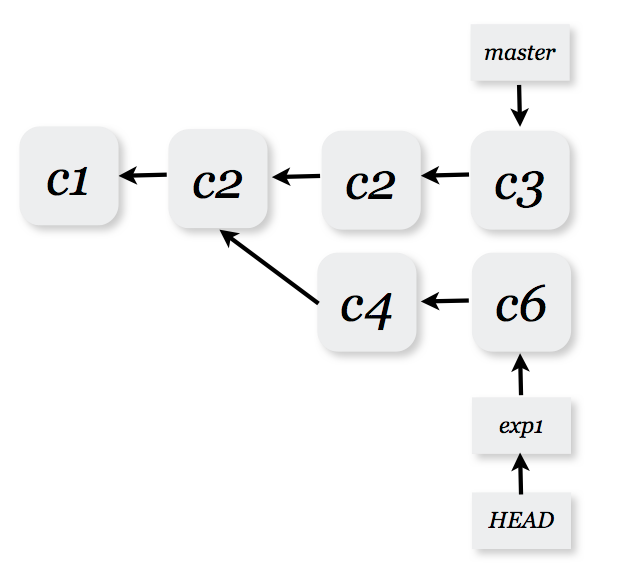
\includegraphics[scale=0.3]{3.png}
    \end{center}
\end{frame}

\begin{frame}[fragile]{Hva er \texttt{rebase}?}
    \setbeamercovered{invisible}
    \begin{lstlisting}[language=bash]
      $ git rebase master
    \end{lstlisting}
    \pause
    \begin{center}
        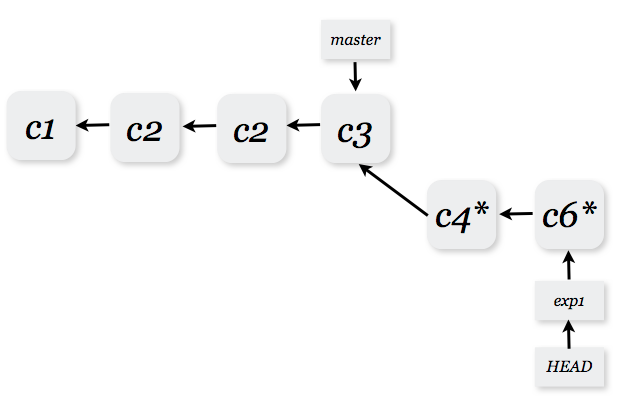
\includegraphics[scale=0.3]{4.png}\\
    \end{center}
\end{frame}

\begin{frame}[fragile]{Hva utgjør en \texttt{commit}?}
    \begin{lstlisting}[language=bash]
       $ git cat-file -p HEAD
       tree 9724058020812154185e7feeed04cb0a8def91d0
       parent 6a72980c6e7010c4687ba65721314d2404047442
       author Pål Ruud <pal.ruud@iterate.no> 1346090316 +0200
       committer Pål Ruud <pal.ruud@iterate.no> 1346090316 +0200

       La til Java-plugin i gradle conf
    \end{lstlisting}
\end{frame}

\begin{frame}{Farlig?}
    \setbeamercovered{invisible}
    Om du rebaser (les: endrer) en commit som finnes på en remote,\\
    vil andre som har basert arbeid på denne committen bli svært forvirret.\\
    \pause
    \bigskip
    \begin{center}
        SÅ IKKE GJØR DET!!1
    \end{center}
\end{frame}

\begin{frame}{Tilbake til det første eksempelet ...}
    \begin{center}
        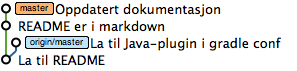
\includegraphics[scale=0.7]{1.png}
    \end{center}
\end{frame}

\begin{frame}[fragile]{Tilbake til det første eksempelet ...}
    \setbeamercovered{invisible}
    \begin{lstlisting}[language=bash]
      $ git pull --rebase
      First, rewinding head to replay your work on top of it...
      Applying: README er i markdown
      Applying: Oppdatert dokumentasjon
    \end{lstlisting}
    \medskip
    \pause
    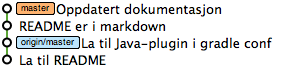
\includegraphics[scale=0.7]{5.png}
\end{frame}

\begin{frame}[fragile]{Hva gjør egentlig \texttt{pull}?}
    \begin{lstlisting}[language=bash]
      $ git pull --rebase origin master
    \end{lstlisting}
    \medskip
    ...er det samme som ...
    \medskip
    \begin{lstlisting}[language=bash]
      $ git fetch
      $ git rebase origin/master
    \end{lstlisting}
\end{frame}

\begin{frame}[fragile]{For den vågale ...}
    \begin{lstlisting}[language=bash, caption=\textasciitilde/.gitconfig]
    [branch]  
      autosetuprebase = always
    \end{lstlisting}
\end{frame}

\begin{frame}{Enkel arbeidsflyt basert på \texttt{rebase}}
    \begin{enumerate}
        \item<+-> Lag ny branch basert på \textbf{master}
        \item<+-> Lag fine, ryddige commits som bare gjør én ting
        \item<+-> Med jevne mellomrom og før sammenslåing, dra ned endringer og rebase på \textbf{master}
        \item<+-> Bytt til \textbf{master} og merge inn feature branch.
    \end{enumerate}
\end{frame}

\begin{frame}{Det er ingen skam å merge...}
    \setbeamercovered{invisible}
    En lineær historie er fint og flott, men noen ganger gir en merge kanskje mening.\\
    \pause
    \medskip
    \begin{itemize}
        \item Ved innhenting av store features til master
        \item Langtlevende featurebrancher som flere utvikler på
    \end{itemize}
    \pause
    (GitHub lager en merge-commit ved lukking av pull request.)
\end{frame}

\begin{frame}{Bonus: \texttt{-{}-interactive}}
    \begin{center}
        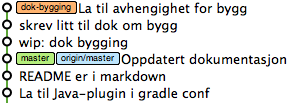
\includegraphics[scale=0.7]{6.png}
    \end{center}
\end{frame}

\begin{frame}[fragile]{Bonus: \texttt{-{}-interactive}}
    \setbeamercovered{invisible}
    \begin{lstlisting}[language=bash]
      $ git rebase -i master
    \end{lstlisting}
    \begin{lstlisting}[language=bash]
pick d342350 wip: dok bygging                             
pick f2b87af skrev litt til dok om bygg                   
pick ee73047 La til avhengighet for bygg                  
                                                          
# Rebase 923acc0..ee73047 onto 923acc0                    
#                                                         
# Commands:                                               
#  p, pick = use commit                                   
#  r, reword = use commit, but edit the commit message    
#  e, edit = use commit, but stop for amending            
#  s, squash = use commit, but meld into previous commit
    \end{lstlisting}
\end{frame}

\begin{frame}[fragile]{Bonus: \texttt{-{}-interactive}}
    \setbeamercovered{invisible}
    \begin{lstlisting}[language=bash]
pick ee73047 La til avhengighet for bygg                  
pick d342350 wip: dok bygging                             
squash f2b87af skrev litt til dok om bygg                   
    \end{lstlisting}
\end{frame}

\begin{frame}[fragile]{Bonus: \texttt{-{}-interactive}}
    \setbeamercovered{invisible}
    \begin{lstlisting}[language=bash]
# This is a combination of 2 commits.                     
# The first commit's message is:                          
                                                          
wip: dok bygging                                          
                                                          
# This is the 2nd commit message:                         
                                                          
skrev litt til dok om bygg 
    \end{lstlisting}
\end{frame}

\begin{frame}{Bonus: \texttt{-{}-interactive}}
    \begin{center}
        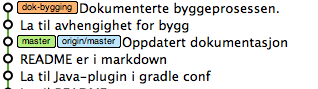
\includegraphics[scale=0.7]{7.png}
    \end{center}
\end{frame}

\setbeamercolor{background canvas}{bg=iterateblue}
\begin{frame}
    \begin{beamercolorbox}[ignorebg]{inverted}
    \begin{center}
        \Huge{git rebase - ta kontrollen over historien}\\
        \vspace{1cm}
        \large{@ruudud \\ https://github.com/ruudud}
    \end{center}
    \end{beamercolorbox}%
\end{frame}
\setbeamercolor{background canvas}{bg=white}

\end{document}
